\documentclass[a4paper,11pt]{article}

% Pakete laden
\usepackage[ngerman]{babel}
\usepackage[utf8]{inputenc}
\usepackage[T1]{fontenc}
\usepackage{geometry}
\usepackage{graphicx}
\usepackage{enumitem}
\usepackage{setspace}
\usepackage{booktabs}
\usepackage{longtable}
\usepackage{multirow}
\usepackage{fancyhdr}
\usepackage{bookmark} 
\usepackage{tocloft}
\usepackage{url}
\usepackage{listings}
\usepackage{xcolor}
\usepackage[hang,flushmargin]{footmisc}

\lstdefinelanguage{TypeScript}{
  language=Java,
  morekeywords={
    interface, implements, private, public, protected, readonly, abstract,
    type, namespace, declare, module, from, as, any, number, boolean, string,
    void, null, undefined, never, unknown
  }
}
\lstset{
  basicstyle=\ttfamily\footnotesize,
  keywordstyle=\color{blue},
  commentstyle=\color{gray},
  stringstyle=\color{red},
  breaklines=true,
  frame=single,
  captionpos=b,
  language=TypeScript
}
\usepackage[scaled=0.92]{helvet}
\renewcommand{\familydefault}{\sfdefault}

\usepackage{hyperref}

\renewcommand{\footnoterule}{\vspace*{0.5em}\hrule width \textwidth height 0.4pt \vspace*{0.6em}}

\geometry{
  top=3.3cm,
  left=2.5cm,
  bottom=2.5cm,
  right=2.5cm,
  headheight=1.8cm,
  footskip=1.3cm
}

\hypersetup{
    bookmarks=true,
    bookmarksnumbered=true,
    colorlinks=true,
    linkcolor=black,
    citecolor=black,
    urlcolor=blue,  
    pdftitle={Dokumentation zur betrieblichen Projektarbeit},
    pdfauthor={Mustafa Shahin},
    pdfsubject={Formular-Editor Schnittstelle},
    pdfkeywords={Angular, Formular-Editor, GSCS},
    pdfstartview={FitH},
    pdfdisplaydoctitle=true
}

\urlstyle{sf}

\singlespacing

\begin{document}

\pagestyle{fancy}
\fancyhf{}
\fancyhead[R]{
\includegraphics[height=1cm]{green_solutions_logo}}
\fancyhead[L]{Formular-Editor Schnittstelle}
\fancyfoot[C]{\thepage}
\renewcommand{\headrulewidth}{0.4pt}
\renewcommand{\footrulewidth}{0.4pt}

\begin{titlepage}
\thispagestyle{empty}

\begin{center}

\includegraphics[width=0.8\textwidth]{ihk_logo}

\vspace{0.5cm}
{\large Abschlussprüfung Sommer 2025}\\
\vspace{0.5cm}
{\large Fachinformatiker für Anwendungsentwicklung}\\
\vspace{1cm}
{\Large\textbf{Dokumentation zur betrieblichen Projektarbeit}}\\
\vspace{1cm}
{\Huge\textbf{Formular-Editor Schnittstelle}}\\
\vspace{0.5cm}
{\Large\textbf{Implementierung eines dynamischen Formular-Editors}}\\
\vspace{0.1cm}
{\Large\textbf{für die GSCS der Green Solutions Software GmbH}}\\
\end{center}

\vspace{0.3cm}
\begin{center}
{\large Abgabedatum: Oldenburg, den 10.05.2025}
\end{center}

\vspace{0.3cm}
\begin{center}
\begin{tabular}{l}
{\large\textbf{Prüfungsbewerber:}}\\
{\large Mustafa Shahin}\\
{\large Grenadierweg 2}\\
{\large 26129 Oldenburg}\\
\\
{\large\textbf{Ausbildungsbetrieb:}}\\
{\large Green Solutions Software GmbH}\\
{\large Eva-Lessing-Straße 6}\\
{\large 26160 Bad Zwischenahn}
\end{tabular}
\end{center}

\begin{center}

\includegraphics[width=0.8\textwidth]{green_solutions_logo}
\end{center}
\end{titlepage}

\tableofcontents
\newpage


\section{Einleitung}
\subsection{Projektumfeld}
Die Green Solutions Software GmbH entwickelt und betreibt die green solutions cloud software (GSCS) als zentrale Software für die grüne Branche\footnote{Grüne Branche: Bezeichnung für den Wirtschaftsbereich, welcher unter anderem Baumschulen und Gartenhäuser beinhaltet.}. Als Teil der kontinuierlichen Weiterentwicklung und Verbesserung der GSCS soll ein dynamischer Formular-Editor entwickelt werden, der es Kunden ermöglicht, eigene Formulare ohne Programmierungskenntnisse zu erstellen und zu verwalten.

\noindent Die GSCS bietet bereits verschiedene vorgefertigte Formulare für unterschiedliche Anwendungsfälle, jedoch erfordert die Anpassung dieser Formulare bisher den Einsatz von Entwicklungsressourcen. Die Entwicklung eines benutzerfreundlichen Formular-Editors würde die Flexibilität der GSCS erhöhen und gleichzeitig Entwicklungsressourcen einsparen.

\subsection{Projektziel}
Ziel des Projekts ist die Implementierung eines dynamischen Formular-Editors als Komponente der GSCS. Der Editor soll es Benutzern ohne Programmierkenntnisse ermöglichen, Formulare nach ihren individuellen Anforderungen zu erstellen und zu gestalten. Die Komponente muss sich nahtlos in die bestehende Architektur der GSCS integrieren und die vorhandenen Designrichtlinien einhalten.

Folgende Kernfunktionalitäten sollen umgesetzt werden:
\begin{itemize}
  \item Drag-and-Drop-Oberfläche zur intuitiven Erstellung von Formularen
  \item Unterstützung verschiedener Eingabefelder (Text, Zahlen, Auswahllisten, etc.)
  \item Responsive Design\footnote{Responsive Design: Ein Ansatz im Webdesign, der sicherstellt, dass Webseiten auf verschiedenen Geräten und Bildschirmgrößen optimal dargestellt werden.} für die optimale Darstellung auf verschiedenen Endgeräten
\end{itemize}

\subsection{Projektbegründung}
Die Implementierung eines dynamischen Formular-Editors für die GSCS bietet mehrere strategische Vorteile:
\begin{itemize}
\item Erstens ermöglicht der Editor den Kunden eine höhere Autonomie bei der Anpassung der Software an ihre individuellen Geschäftsprozesse. Dies steigert die Flexibilität und Akzeptanz der GSCS bei bestehenden und potenziellen Kunden.

\item Zweitens reduziert die Self-Service-Funktionalität den Support- und Entwicklungsaufwand für die GSS-GmbH. Statt individuelle Formularanpassungen durch Entwickler vornehmen zu lassen, können Kunden diese Anpassungen selbständig durchführen.

\item Drittens ermöglicht der Editor eine schnellere Reaktion auf sich ändernde gesetzliche Anforderungen oder Marktbedingungen, da Anpassungen an Formularen zeitnah ohne Programmieraufwand erfolgen können.

\noindent Die Entwicklung eines neuen Formular-Editors ist auch durch einen wichtigen technologischen Wandel begründet: Die GSCS befindet sich derzeit in einer umfassenden Frontend-Modernisierung. Das bestehende Formular-Builder-System wurde ursprünglich mit DOTNET\footnote{DOTNET: Web-Framework von Microsoft zur serverseitigen Entwicklung dynamischer Webseiten und Webanwendungen.} und jQuery\footnote{jQuery: JavaScript-Bibliothek zur Vereinfachung von DOM-Manipulation, Events und Ajax-Anfragen.} entwickelt, während die neue Frontend-Anwendung vollständig auf Angular\footnote{Angular: Moderne TypeScript-basierte Webframework von Google für die Entwicklung dynamischer Single-Page-Anwendungen.} und Tailwind CSS\footnote{Tailwind CSS: Utility-First CSS-Framework zur schnellen Gestaltung von Benutzeroberflächen direkt im HTML-Code.} basiert.

\end{itemize}
\subsection{Projektschnittstellen}

Die Formular-Editor-Komponente interagiert mit verschiedenen Schnittstellen innerhalb der GSCS:

\noindent \textbf{Technische Schnittstellen:} Die Komponente wird in Angular entwickelt und kommuniziert mit dem DOTNET-Backend der GSCS über REST-APIs\footnote{REST-API: Schnittstelle, die auf dem HTTP-Protokoll basiert und einen einfachen, standardisierten Datenaustausch zwischen Client und Server ermöglicht.}. Die Formularstrukturen werden in der SQL-Datenbank der GSCS gespeichert. Die Darstellung der Formulare erfolgt über die neu entwickelte GSCS Frontend-App, die auf Angular und Tailwind CSS basiert.


\noindent \textbf{Organisatorische Schnittstellen:} Die Entwicklung erfolgt in Abstimmung mit dem Frontend-Team und dem Backend-Team der GSS-GmbH. Der Projektfortschritt wird in regelmäßigen Abständen mit dem Abteilungsleiter Entwicklung besprochen. Die Abnahme des Projekts erfolgt durch den TEamleiter, einen Senior-Frontend-Entwickler und die Geschäftsführung.

\noindent \textbf{Benutzergruppen:} Primäre Benutzergruppen sind Administratoren und Power-User auf Kundenseite, die eigene Formulare erstellen und verwalten werden. Sekundäre Benutzergruppen sind die Endanwender, die die erstellten Formulare ausfüllen werden.

\subsection{Projektmethodik}
Die Implementierung des Formular-Editors erfolgte streng nach dem Wasserfallmodell, einer sequentiellen Projektmanagement-Methode, die durch klar definierte und aufeinanderfolgende Phasen gekennzeichnet ist. Diese Methodik wurde aufgrund der gut definierten Anforderungen und des überschaubaren Projektumfangs gewählt.

Der Entwicklungsprozess umfasste folgende strikt voneinander getrennte Phasen:
\begin{enumerate}
  \item \textbf{Anforderungsanalyse}: Detaillierte Erfassung aller funktionalen und nicht-funktionalen Anforderungen, die vollständig abgeschlossen wurde, bevor die Design-Phase begann
  \item \textbf{Design}: Entwurf der Systemarchitektur und der Benutzeroberfläche, wobei alle Design-Entscheidungen vor Beginn der Implementierung finalisiert wurden
  \item \textbf{Implementierung}: Umsetzung des Designs in funktionierenden Code, basierend ausschließlich auf den in der Design-Phase festgelegten Spezifikationen
  \item \textbf{Test}: Umfassende Überprüfung der Funktionalität und Qualitätssicherung nach Abschluss der Implementierung
  \item \textbf{Abnahme}: Finaler Test und Abnahme durch Stakeholder
  \item \textbf{Deployment}: Bereitstellung der Lösung im Produktivsystem
  \item \textbf{Wartung}: Fortlaufende Pflege und Erweiterung der Komponente
\end{enumerate}

\noindent Diese strukturierte Vorgehensweise ermöglichte eine klare Planung und Kontrolle des Projektfortschritts sowie eine gründliche Dokumentation in jeder Phase. Das Qualitätssicherungs- und Feedbackverfahren erfolgte entsprechend dem Wasserfallmodell in der dafür vorgesehenen Testphase, um die Einhaltung der initial definierten Anforderungen zu gewährleisten.

\subsection{Projektabgrenzung}
Der Formular-Editor wird als Komponente in die bestehende GSCS integriert und nutzt die vorhandene Infrastruktur. Folgende Aspekte sind nicht Teil des Projekts:

\begin{itemize}
  \item Entwicklung einer eigenständigen Formular-Editor-Anwendung außerhalb der GSCS
  \item Bestehende Formulare: Diese verbleiben im alten System, und neue Formulare werden mit dem neuen Editor erstellt
\end{itemize}

\noindent Für das Speichern und Laden von Formularstrukturen werden die existierenden Datenbankstrukturen verwendet. Die Formularstruktur wird im JSON\footnote{JSON (JavaScript Object Notation): Leichtgewichtiges Datenformat zur strukturierten Datenübertragung, das insbesondere im Web-Umfeld weit verbreitet ist.}-Format in einer eigenen Spalte in der bestehenden Formulartabelle gespeichert, wobei das JSON-Schema komplexe TypeScript\footnote{TypeScript: Eine statisch typisierte Programmiersprache, die auf JavaScript aufbaut und die Entwicklung durch Typsicherheit und erweiterte Features unterstützt.}-Interfaces wie FormField abbildet, die IDs, Typen, Spaltenbreiten und weitere Metadaten enthalten.


\section{Analyse}
\subsection{Durchführung der Ist-Analyse}
Die aktuelle Situation bezüglich der Formularerstellung und -verwaltung in der GSCS wurde anhand von Interviews mit Kunden, Support-Mitarbeitern und Entwicklern analysiert.

\noindent Aktuell bietet die GSCS eine begrenzte Anzahl vordefinierter Formulare für verschiedene Anwendungsfälle. Diese Formulare sind statisch und können nur durch Entwickler angepasst werden. Kundenspezifische Anpassungen erfordern daher einen Entwicklungsauftrag, der sowohl Zeit- als auch Kostenaufwand für den Kunden bedeutet.

Der aktuelle Prozess zur Anpassung von Formularen umfasst folgende Schritte:
\begin{enumerate}
  \item Der Kunde formuliert seine Anforderungen an das Formular
  \item Ein Entwickler implementiert die Änderungen im Quellcode
  \item Die Änderungen durchlaufen den Qualitätssicherungsprozess
  \item Die angepasste Version wird im Rahmen eines regulären Releases ausgeliefert
\end{enumerate}

\noindent Dieser Prozess dauert je nach Komplexität der Anforderungen und Auslastung der Entwicklungsabteilung zwischen einer und zwei Wochen, da aufgrund der begrenzten Ressourcen in der Entwicklungsabteilung nicht alle Kundenanforderungen zeitnah umgesetzt werden können, was zu Unzufriedenheit führt.

\subsection{Durchführung der Soll-Analyse}
Basierend auf den Erkenntnissen der Ist-Analyse und den Anforderungen der Stakeholder wurden folgende Anforderungen an den Formular-Editor definiert:

\textbf{Funktionale Anforderungen:}
\begin{itemize}
  \item Intuitive Drag-and-Drop-Oberfläche zur Erstellung und Bearbeitung von Formularen
  \item Unterstützung folgender Feldtypen: Text, E-Mail, Passwort, Zahl, DatePicker (Datum), TimePicker (Zeit), Select (Auswahlliste), Checkbox, FileUpload (Datei-Upload), TextArea (Textbereich)
  \item Konfigurationsmöglichkeiten für jedes Feld: Label, Platzhaltertext, Standardwert, Pflichtfeld-Markierung
  \item Responsives Design für verschiedene Bildschirmgrößen
  \item Anpassbare Formularlayouts mit Spalten und Abschnitten
\end{itemize}

\textbf{Nicht-funktionale Anforderungen:}
\begin{itemize}
  \item Benutzerfreundlichkeit: Der Editor muss ohne technische Vorkenntnisse bedienbar sein
  \item Performance: Die Ladezeit für den Editor darf 5 Sekunden nicht überschreiten
  \item Sicherheit: Einhaltung der DSGVO-Anforderungen
  \item Wartbarkeit: Modularer Aufbau für einfache Erweiterbarkeit
\end{itemize}

\subsection{Wirtschaftlichkeitsanalyse und Amortisationsrechnung}
\subsubsection{Make-or-Buy Entscheidung}
Für die Implementierung des Formular-Editors wurden drei Optionen in Betracht gezogen:

\begin{enumerate}
  \item Entwicklung einer Eigenimplementierung
  \item Integration einer Open-Source-Lösung
  \item Kauf einer kommerziellen Lösung
\end{enumerate}

\noindent Nach einer gründlichen Analyse der verfügbaren Optionen wurde die Entscheidung für eine Eigenimplementierung getroffen. Die Gründe hierfür waren:

\begin{itemize}
  \item Bessere Integration in die bestehende GSCS-Architektur
  \item Volle Kontrolle über Funktionsumfang und Anpassbarkeit
  \item Keine Lizenzkosten für Drittanbieter-Lösungen
  \item Vorhandenes Know-how im Entwicklungsteam für diese Art von Komponenten
  \item Spezifische Anforderungen der grünen Branche, die von Standardlösungen nicht abgedeckt werden
\end{itemize}

\noindent Obwohl die Entwicklungsabteilung im Tagesgeschäft durch zahlreiche Kundenanfragen ausgelastet ist, verfügt sie über das notwendige Fachwissen für die Eigenentwicklung dieser Komponente. Die Entscheidung zur Eigenentwicklung wurde getroffen, um langfristig Ressourcen zu sparen, da die Formularanpassungen nach Projektabschluss nicht mehr durch die Entwicklungsabteilung durchgeführt werden müssen.

\noindent Die untersuchten Open-Source-Lösungen erfüllten nicht alle Anforderungen oder hätten erhebliche Anpassungen erfordert. Kommerzielle Lösungen waren mit hohen Lizenzkosten verbunden und boten ebenfalls keine optimale Integration in die GSCS..

\subsubsection{Projektkosten}
\noindent Der Personalaufwand wurde mit 40 Arbeitsstunden für die Implementierung und Testen des Formular-Editors angesetzt. Der durchschnittliche Stundensatz für Entwickler (Auszubildende) beträgt 30€/Stunde. Die Dokumentation und Schulung umfasst 40 Stunden.

\begin{table}[h]
\centering
\begin{tabular}{lrrr}
\toprule
\textbf{Position} & \textbf{Stunden} & \textbf{Stundensatz} & \textbf{Kosten} \\
\midrule
Entwicklung & 40 & 30€ & 1.200€ \\
Dokumentation/Schulung & 40 & 30€ & 1.200€ \\
\midrule
\textbf{Gesamtkosten} & & & \textbf{2.400€} \\
\bottomrule
\end{tabular}
\caption{Kostenkalkulation für die Implementierung des Formular-Editors}
\end{table}

\noindent Für die Umsetzung des Projekts wird folgende Hardware verwendet: Ein leistungsstarker Arbeitsplatzrechner mit sechs Bildschirmen für das Büro sowie ein weiterer PC mit drei Bildschirmen für den Einsatz im Homeoffice. Als Software kommen Windows 11 Professional, Visual Studio 2022 Professional, Visual Studio Code sowie GitHub Enterprise zum Einsatz, um eine effiziente und professionelle Entwicklungsumgebung sicherzustellen.

\subsubsection{Amortisationsdauer}
Zur Berechnung der Amortisationsdauer wurden die Projektkosteneinsparungen durch den Formular-Editor analysiert. Basierend auf historischen Daten bearbeitet die Entwicklungsabteilung durchschnittlich 15 Formularanpassungen pro Monat mit einem durchschnittlichen Aufwand von 4 Stunden pro Anpassung. Bei einem Stundensatz von 65€ entspricht dies monatlichen Kosten von 3.900€.

\noindent Mit dem Formular-Editor können Kunden Anpassungen selbst vornehmen, was den Entwicklungsaufwand reduziert. Es wird erwartet, dass 80\% der Formularanpassungen von Kunden selbst durchgeführt werden können. Dies führt zu einer monatlichen Einsparung von 3.120€.


\noindent Bei einer Investition von 2.400€ und monatlichen Einsparungen von 3.120€ beträgt die Amortisationszeit etwa 0,8 Monate (2.400€ ÷ 3.120€, gerundet 0,8). Die schnelle Amortisation bestätigt die wirtschaftliche Vorteilhaftigkeit des Projekts.

\section{Entwurf}
\subsection{Verfügbare Datensätze ermitteln}
Als Grundlage für den Entwurf des Formular-Editors wurde zunächst eine Analyse der in der GSCS verfügbaren Datenstrukturen durchgeführt. Dies umfasste die Identifikation der relevanten Entitäten und deren Beziehungen zueinander.

\noindent Die GSCS verfügt bereits über eine Tabelle für Formulare, die um zusätzliche Spalten für die Formularstruktur erweitert werden kann. Ein Formular in der GSCS besteht aus folgenden Hauptkomponenten:

\begin{itemize}
  \item Formular-Metadaten (Titel, Beschreibung, Erstellungsdatum, letzte Änderung)
  \item Formularfelder mit Konfigurationen
  \item Layout-Informationen (Anordnung der Felder, Spalten, Abschnitte)
\end{itemize}

\noindent Für die Darstellung der Formularfelder im Editor wurden die bestehenden UI-Komponenten der GSCS analysiert. Dabei hat sich gezeigt, dass einige der benötigten Komponenten bereits im Design-System vorhanden sind und wiederverwendet werden können, während weitere Komponenten neu entwickelt werden müssen. Zusätzlich wird ein Service erstellt, um die Verwaltung der Formular-Komponenten zu übernehmen und eine konsistente Darstellung sicherzustellen.

\subsection{Entwurf der Datenmodellumwandlung}
Für die Speicherung der Formularstrukturen wurde ein flexibles JSON-Schema entworfen, das alle erforderlichen Informationen enthält. Das Schema umfasst folgende Hauptbereiche:

\begin{itemize}
  \item Form-Metadaten: Allgemeine Informationen wie Titel, Beschreibung und Erstellungsdatum
  \item Grid-Layout\footnote{Grid-System: Ein Layout-Framework, das auf einer Reihe von Zeilen und Spalten basiert, um Inhalte zu organisieren. Typischerweise basiert es im modernen Webdesign auf 12 Spalten.}: Definition der Zeilen und Spalten für die Platzierung der Formularfelder
  \item Felder: Detaillierte Informationen zu jedem Formularfeld, einschließlich Typ, Label.
\end{itemize}

\noindent Das JSON-Schema ermöglicht eine flexible Erweiterung um neue Feldtypen oder Konfigurationsoptionen, ohne Änderungen an der Datenbankstruktur vornehmen zu müssen. Ein Beispiel für das Schema befindet sich im Anhang.

\noindent Um eine effiziente Bearbeitung von Formularen im Frontend zu ermöglichen, wurde ein Formularmodell für Angular entwickelt, das die Konvertierung zwischen dem JSON-Schema und den TypeScript-Objekten übernimmt. Dies vereinfacht die Implementierung des Drag-and-Drop-Editors und die Validierung der Formularstruktur.


\subsection{Technischer Entwurf der Schnittstelle}
Der Formular-Editor besteht aus mehreren Hauptkomponenten, die miteinander interagieren:

\begin{itemize}
  \item Form-Canvas: Der Hauptbereich, in dem das Formular per Drag-and-Drop gestaltet wird
  \item Jedes Formularfeld kann durch einen Resize-Handle an der rechten Seite in seiner Breite verändert werden. Die Implementierung nutzt die Bibliothek 'angular-resizable-element', um eine intuitive Größenänderung zu ermöglichen.
  \item Ein zentraler BuilderService wurde implementiert, der die Layout-Berechnungen, Drag-and-Drop-Operationen und Validierung der Formularstruktur übernimmt.
  \item Field-Sidebar: Eine Seitenleiste mit verfügbaren Formularfeldern, die per Drag-and-Drop auf den Canvas gezogen werden können
  \item Properties-Panel: Ein Bereich zur Konfiguration der Eigenschaften des ausgewählten Formularfelds
\end{itemize}

\noindent Der Form-Canvas nutzt ein auf 12 Spalten basierendes Grid-System. Jedes Formularfeld verfügt über eine columns-Eigenschaft, die angibt, wie viele dieser Spalten es beansprucht. Der BuilderService ermittelt automatisch die verbleibenden Platzkapazitäten und passt das Layout dynamisch entsprechend an.

\noindent Die Kommunikation zwischen den Komponenten erfolgt über Angular-Services\footnote{Angular-Services: Singleton-Objekte in Angular-Anwendungen, die spezifische Funktionalitäten über Komponenten hinweg bereitstellen, oft für Datenaustausch und Geschäftslogik verwendet.}, die den Zustand des Formulars verwalten und Änderungen an alle beteiligten Komponenten propagieren. Für die Drag-and-Drop-Funktionalität wird die Bibliothek ngx-drag-drop\footnote{ngx-drag-drop: Eine Angular-Bibliothek, die Drag-and-Drop-Funktionalität mit einer einfachen und intuitiven API zur Verfügung stellt.} verwendet.
\noindent Die Speicherung der Formulare erfolgt über REST-API-Calls an das Backend. Die API-Schnittstelle wurde so gestaltet, dass sie Speichervorgang unterstützt.

\noindent Die Internationalisierung wird vollständig durch das Modul ngx-translate\footnote{ngx-translate: Eine Angular-Bibliothek zur Implementierung von Mehrsprachigkeit in Anwendungen, die es ermöglicht, Texte und UI-Elemente dynamisch in verschiedenen Sprachen anzuzeigen.} unterstützt, wodurch alle Texte und Beschriftungen lokalisiert werden können.
\section{Implementierung}
\subsection{Initialisierung des Projekts}
Die Implementierung begann mit der Einrichtung der Entwicklungsumgebung und der Definition der grundlegenden Projektstruktur. Da der Formular-Editor als Komponente in die bestehende GSCS integriert werden sollte, wurde ein neues Angular-Modul innerhalb des bestehenden Projekts erstellt.

\noindent Die Projektstruktur folgt den Best Practices für Angular-Anwendungen und orientiert sich an der bereits etablierten Struktur der GSCS. Die Hauptkomponenten wurden als eigenständige Module implementiert, um eine klare Trennung der Verantwortlichkeiten zu gewährleisten und die Wiederverwendbarkeit zu fördern.

\noindent Für die Versionskontrolle wurde ein dedizierter Branch im GitHub\footnote{GitHub: Eine cloudbasierte Plattform für Softwareentwicklung, die auf Git basiert und zusätzliche Funktionen für Teamarbeit, Code-Reviews und kontinuierliche Integration bietet.}-Repository\footnote{Repository: Ein zentraler Speicherort in der Versionskontrolle, in dem der Quellcode eines Projekts und dessen gesamte Änderungshistorie gespeichert werden.} der GSCS erstellt, um die parallele Entwicklung zu ermöglichen, ohne den Hauptentwicklungszweig zu beeinträchtigen.

\subsection{Implementierung der Modellumwandlung}
Die Implementierung der Modellumwandlung umfasste die Erstellung von TypeScript-Interfaces und Klassen zur Repräsentation der Formularstruktur im Frontend. Diese Modelle bilden die Grundlage für die Interaktion zwischen dem Benutzer und der Formularstruktur.

\noindent Ein zentraler Service wurde implementiert, der die Konvertierung zwischen dem JSON-Schema und den TypeScript-Objekten übernimmt. Dieser Service ist auch für die Validierung der Formularstruktur verantwortlich und stellt sicher, dass nur gültige Formulare gespeichert werden können.

\noindent Die Modellklassen enthalten Methoden zur Manipulation der Formularstruktur, wie das Hinzufügen und Entfernen von Feldern, das Ändern von Feldeigenschaften und das Anpassen des Layouts. Diese Methoden werden von den UI-Komponenten aufgerufen, um Benutzeraktionen zu verarbeiten.


\subsection{Implementierung der automatischen Abläufe}
Zur Unterstützung des Formular-Editors wurden mehrere automatische Abläufe implementiert, die die Benutzererfahrung verbessern und die Konsistenz der Daten gewährleisten:

\begin{itemize}
  \item Automatisches Speichern: Der Editor speichert den aktuellen Zustand des Formulars regelmäßig als Entwurf, um Datenverlust zu verhindern
  \item Layout-Anpassung: Bei Änderungen an der Größe oder Position eines Felds werden andere Felder automatisch angepasst, um Überlappungen zu vermeiden
  \item Validierung: Bei jeder Änderung wird die Formularstruktur validiert, um ungültige Zustände zu vermeiden
\end{itemize}

\noindent Diese automatischen Abläufe wurden als Teil der Angular-Services implementiert und sind eng mit dem Zustandsmanagement des Editors verbunden.

\subsection{Integration in das bestehende System}
Die Integration des Formular-Editors in die bestehende GSCS erforderte eine sorgfältige Abstimmung mit anderen Komponenten und Modulen. Folgende Integrationsschritte wurden durchgeführt:

\begin{itemize}
  \item Einbindung in das Menüsystem der GSCS zur Navigation zum Formular-Editor
  \item Integration in das Berechtigungssystem zur Steuerung des Zugriffs auf den Editor
  \item Anpassung des bestehenden Formular-Renderers zur Darstellung der mit dem Editor erstellten Formulare
\end{itemize}

\noindent Die Integration wurde schrittweise durchgeführt und nach jedem Schritt gründlich getestet, um Kompatibilitätsprobleme frühzeitig zu erkennen und zu beheben.

\subsection{Implementierung der Konfiguration}
Um eine hohe Flexibilität und Anpassbarkeit des Formular-Editors zu gewährleisten, wurde ein umfassendes Konfigurationssystem implementiert. Dieses System ermöglicht die Anpassung des Editors an verschiedene Anwendungsfälle und Kundenanforderungen, ohne den Quellcode ändern zu müssen.

\noindent Die Konfiguration umfasst folgende Bereiche:
\begin{itemize}
  \item Layout-Optionen: Konfiguration der verfügbaren Spaltenbreiten und Layoutvarianten
  \item Erscheinungsbild: Anpassung des Designs an das Corporate Design des Kunden
\end{itemize}

\noindent Die Konfigurationsoptionen werden in der Datenbank gespeichert und beim Start des Editors geladen. Änderungen an der Konfiguration werden sofort wirksam, ohne dass ein Neustart der Anwendung erforderlich ist.

\section{Abnahme}
\subsection{Initiales Deployment auf einem Testsystem}
Nach Abschluss der Implementierung wurde der Formular-Editor auf einem Testsystem deployt, um eine umfassende Validierung der Funktionalität und Integration durchzuführen. Das Testsystem ist eine Kopie des Produktivsystems mit realistischen Testdaten, um möglichst produktionsnahe Bedingungen zu simulieren.

\noindent Für das Deployment wurden die in der GSCS etablierten CI/CD\footnote{CI/CD: Continuous Integration und Continuous Deployment, eine Entwicklungspraxis, bei der Codeänderungen automatisch getestet und in die Produktionsumgebung übertragen werden.}-Prozesse verwendet, die eine automatisierte Bereitstellung und Konfiguration der Anwendung ermöglichen. Nach dem Deployment wurde eine initiale Konfiguration des Editors vorgenommen, um die grundlegende Funktionalität zu überprüfen.

\noindent Der Deploymentprozess wurde detailliert dokumentiert, um eine reibungslose Bereitstellung auf anderen Umgebungen zu gewährleisten.

\subsection{Übertragungstests}
Nach dem initialen Deployment wurden umfangreiche Tests durchgeführt, um die Funktionalität des Formular-Editors zu validieren. Die Tests umfassten folgende Bereiche:

\begin{itemize}
  \item Funktionale Tests: Überprüfung aller Funktionen des Editors gemäß den Anforderungen
  \item Integrationstests: Validierung der Integration mit anderen Komponenten der GSCS
  \item Usability-Tests: Bewertung der Benutzerfreundlichkeit durch potenzielle Endbenutzer
  \item Performance-Tests: Messung der Ladezeiten und Reaktionsgeschwindigkeit
  \item Sicherheitstests: Überprüfung auf potenzielle Sicherheitslücken
\end{itemize}

\noindent Die Tests wurden sowohl manuell als auch automatisiert durchgeführt. Für die automatisierten Tests wurden Cypress und Jest verwendet, um eine hohe Testabdeckung zu erreichen und Regressionstests zu ermöglichen.

\noindent Während der Tests wurden einige Probleme identifiziert, insbesondere bei der Performanz bei komplexen Formularen und bei der Benutzerfreundlichkeit bestimmter Interaktionen. Diese Probleme wurden dokumentiert und in der Implementierung behoben.

\subsection{Initiales Deployment auf dem Produktivsystem}
Nach erfolgreicher Validierung auf dem Testsystem wurde der Formular-Editor auf dem Produktivsystem deployt. Der Deploymentprozess folgte dem gleichen Verfahren wie beim Testsystem, mit zusätzlichen Sicherheitsmaßnahmen aufgrund der höheren Kritikalität des Produktivsystems.

\noindent Das Deployment wurde in einer Phase mit geringer Benutzeraktivität durchgeführt, um potenzielle Auswirkungen auf den laufenden Betrieb zu minimieren. Nach dem Deployment wurde eine umfassende Funktionsprüfung durchgeführt, um sicherzustellen, dass alle Funktionen wie erwartet arbeiten.

\noindent Den ersten Benutzern wurde der Zugriff auf den Editor schrittweise gewährt, beginnend mit einer Pilotgruppe, um Feedback zu sammeln und potenzielle Probleme zu identifizieren, bevor die Funktion allen Benutzern zur Verfügung gestellt wurde.

\subsection{Tests mit Realdaten}
Nach dem Deployment auf dem Produktivsystem wurden Tests mit realen Kundendaten durchgeführt, um sicherzustellen, dass der Formular-Editor unter realen Bedingungen korrekt funktioniert. Diese Tests umfassten:

\begin{itemize}
  \item Erstellung vollständig neuer Formulare basierend auf aktuellen Anforderungen der Kunden
  \item Test der neu erstellten Formulare mit realen Daten aus dem Tagesgeschäft
  \item Überprüfung der Datenvalidierung und -speicherung
\end{itemize}

\noindent Die Tests bezogen sich ausschließlich auf neu erstellte Formulare. Die bestehenden Formulare aus dem alten System bleiben unverändert und werden nicht in den neuen Formular-Editor übertragen. Stattdessen werden Kunden bei Bedarf neue Formulare mit dem Editor erstellen.

\noindent Die Tests mit Realdaten bestätigten die grundlegende Funktionalität des Editors und lieferten wertvolles Feedback für zukünftige Verbesserungen. Diese abschließende Testphase erfolgte gemäß dem Wasserfallmodell erst nach vollständiger Implementierung und steht im Einklang mit der sequentiellen Projektmethodik.

\section{Interne Dokumentation}
\subsection{Entwicklerdokumentation}
Zur Unterstützung der zukünftigen Wartung und Weiterentwicklung des Formular-Editors wurde eine umfassende Entwicklerdokumentation erstellt. Diese Dokumentation besteht aus mehreren Teilen:

\begin{itemize}
  \item Architekturübersicht: Beschreibung der Gesamtarchitektur und der Interaktion der verschiedenen Komponenten
  \item Komponentendokumentation: Detaillierte Beschreibung jeder Komponente, ihrer Verantwortlichkeiten und Schnittstellen
  \item Datenmodell: Detaillierte Beschreibung des Datenmodells und der Datenbankstruktur
  \item Erweiterungsleitfaden: Anleitung zur Erweiterung des Editors um neue Feldtypen oder Funktionen
\end{itemize}

\noindent Die Dokumentation wurde in Markdown\footnote{Markdown: Eine einfache Auszeichnungssprache, die leicht zu lesen und zu schreiben ist und in einfaches HTML konvertiert werden kann. Markdown wird häufig für Dokumentation und in Wikis verwendet, da es die Erstellung von strukturierten Dokumenten ohne komplexe Formatierungsbefehle ermöglicht.} erstellt und im internen Wiki der GSS-GmbH veröffentlicht. Zusätzlich wurden die relevanten Codeabschnitte mit ausführlichen Kommentaren versehen, um das Verständnis und die Wartbarkeit des Codes zu verbessern.

\noindent Die Entwicklerdokumentation wurde mit dem Entwicklungsteam abgestimmt und in einem Review-Prozess validiert, um sicherzustellen, dass alle relevanten Aspekte abgedeckt sind und die Dokumentation verständlich und vollständig ist.

\subsection{Benutzerhandbuch}
Neben der Entwicklerdokumentation wurde ein umfassendes Benutzerhandbuch erstellt, das sich an die Endbenutzer des Formular-Editors richtet. Das Benutzerhandbuch enthält folgende Abschnitte:

\begin{itemize}
  \item Einführung: Übersicht über den Formular-Editor und seine Funktionen
  \item Erste Schritte: Anleitung zur ersten Nutzung des Editors
  \item Grundlegende Funktionen: Erstellung, Bearbeitung und Verwaltung von Formularen
  \item Feldtypen: Beschreibung der verfügbaren Feldtypen und ihrer Eigenschaften
  \item Layout-Gestaltung: Anleitung zur Gestaltung des Formularlayouts
  \item Beispiele: Schrittweise Anleitungen für typische Anwendungsfälle
  \item Fehlerbehebung: Lösungen für häufige Probleme
\end{itemize}

\noindent Das Benutzerhandbuch wurde mit zahlreichen Screenshots und Beispielen angereichert, um die Verständlichkeit zu erhöhen. Entsprechend der Wasserfallmethodik wurde das Handbuch nach Abschluss der Implementierungsphase erstellt und anschließend durch ausgewählte Testbenutzer validiert. Die Rückmeldungen der Testbenutzer wurden gesammelt und für die finale Version des Handbuchs berücksichtigt, ohne dabei den sequentiellen Entwicklungsprozess zu unterbrechen.


\section{Fazit}
\subsection{Soll-/Ist-Vergleich}
Die Implementierung des Formular-Editors wurde größtenteils gemäß den ursprünglichen Anforderungen und dem geplanten Zeitrahmen abgeschlossen. Ein detaillierter Vergleich der Soll- und Ist-Werte zeigt sowohl Erfolge als auch Herausforderungen des Projekts.\\
\\
\noindent \textbf{Funktionsumfang:} Alle in der Anforderungsanalyse definierten Kernfunktionen wurden erfolgreich implementiert. Einige weniger kritische Funktionen, wie das Speichern von Vorlagen, wurde aufgrund von Zeitbeschränkungen auf eine spätere Version verschoben.\\
\\
\noindent \textbf{Zeitplan:} Das Projekt wurde planmäßig ohne Verzögerung abgeschlossen. Trotz technischer Herausforderungen bei der Integration des Drag-and-Drop-Systems mit dem responsiven Grid-Layout und potenzieller Komplikationen bei der Validierung komplexer Formulare konnte der ursprüngliche Zeitplan eingehalten werden. Dies hatte entsprechend positive Auswirkungen auf die geplante Release-Planung.\\
\\
\noindent \textbf{Qualität:} Die Qualitätsziele des Projekts wurden weitgehend erreicht. Die Benutzerfreundlichkeit wurde in den Tests mit durchschnittlich 4,2 von 5 Punkten bewertet, was über dem Zielwert von 4,0 liegt. Die in den nicht-funktionalen Anforderungen festgelegte Ladezeit von maximal 5 Sekunden wurde für einfache und mittelschwere Formulare vollständig erreicht.\\
\\

\noindent \textbf{Benutzerakzeptanz:} Die ersten Rückmeldungen von Benutzern nach dem Release waren überwiegend positiv. Insbesondere wurde die intuitive Bedienung und die Flexibilität bei der Gestaltung von Formularen gelobt.

\subsection{Ausblick}
Basierend auf den Erfahrungen und dem Feedback aus der ersten Version des Formular-Editors wurden mehrere Ansatzpunkte für zukünftige Erweiterungen und Verbesserungen identifiziert:

\begin{itemize}
  \item Optimierung der Performance bei komplexen Formularen durch verbesserte Rendering-Algorithmen
  \item Erweiterung um zusätzliche Feldtypen, wie z.B. Signaturfeld, Rating-Skala und Datums-Range
  \item Implementierung erweiterter Validierungsregeln, einschließlich konditionale Validierung basierend auf anderen Feldern
  \item Implementierung einer Vorlagenbibliothek mit branchenspezifischen Formularvorlagen
  \item Erweiterung um Mehrsprachigkeit für internationale Kunden
\end{itemize}

\noindent Für die nächste Version ist bereits ein Feature-Set definiert, das auf Basis der Prioritätsbewertung durch Produktmanagement und Kundenfeedback ausgewählt wurde. Die Entwicklung dieser Version ist für das kommende Quartal geplant.

\noindent Langfristig wird der Formular-Editor zu einem zentralen Bestandteil der GSCS ausgebaut, der nicht nur für eigenständige Formulare, sondern auch für die Konfiguration von Eingabemasken in anderen Modulen der GSCS genutzt werden kann. Dies wird zu einer einheitlichen Benutzererfahrung über die gesamte Anwendung hinweg beitragen und die Flexibilität für Kunden weiter erhöhen.

\subsection{Gelerntes}
Bei der Entwicklung des Formular-Editors Komponante und seiner Services habe ich viel gelernt, sowohl in technischer als auch in projektorganisatorischer Hinsicht.

\paragraph{Technische Erkenntnisse}
Im technischen Bereich konnte ich meine Kenntnisse in Angular und der Entwicklung komplexer, interaktiver Benutzeroberflächen vertiefen. Insbesondere die Implementierung des Drag-and-Drop-Systems in Verbindung mit einem responsiven Grid-Layout stellte eine interessante Herausforderung dar, die eine tiefe Auseinandersetzung mit den Möglichkeiten von Angular und dem Angular ngx-drag-drop erforderte.

\noindent Die Erstellung eines flexiblen JSON-Schemas zur Speicherung der Formularstrukturen hat mir wertvolle Einblicke in die Datenmodellierung und die Vor- und Nachteile verschiedener Ansätze zur Speicherung komplexer, hierarchischer Daten gegeben. Die Notwendigkeit, ein System zu entwerfen, das sowohl erweiterbar als auch performant ist, führte zu wichtigen Erkenntnissen über die Balance zwischen Flexibilität und Komplexität.

\paragraph{Projektmanagement-Erkenntnisse}
Aus projektorganisatorischer Sicht war die systematische Einhaltung des Wasserfallmodells während der gesamten Projektlaufzeit eine wertvolle Erfahrung. Die klare Trennung der Entwicklungsphasen und die ausführliche Dokumentation nach jeder abgeschlossenen Phase haben wesentlich zum Erfolg des Projekts beigetragen. Insbesondere die detaillierte Anforderungsanalyse zu Beginn des Projekts hat sich als entscheidend für die effiziente Durchführung der nachfolgenden Phasen erwiesen. Auch das strukturierte Vorgehen in der Testphase, bei dem alle Funktionen systematisch überprüft wurden, hat zur hohen Qualität des Endprodukts beigetragen.

\paragraph{Wirtschaftliche Erkenntnisse}
Die Durchführung der Wirtschaftlichkeitsanalyse und die Berechnung der Amortisationszeit haben mir ein besseres Verständnis für die ökonomischen Aspekte der Softwareentwicklung vermittelt. Die Erkenntnis, dass eine sorgfältige Analyse der langfristigen Kosten und Einsparungen für die Bewertung eines Projekts ebenso wichtig ist wie die technische Umsetzbarkeit, wird meine zukünftige Arbeit beeinflussen.

\paragraph{Dokumentation}
Nicht zuletzt hat mir das Projekt die Bedeutung einer gründlichen Dokumentation vor Augen geführt. Die Investition in eine umfassende und verständliche Dokumentation erleichtert nicht nur die zukünftige Wartung und Weiterentwicklung, sondern trägt auch wesentlich zur Akzeptanz und erfolgreichen Nutzung durch die Endanwender bei. Die strikte Trennung zwischen Entwickler- und Benutzerdokumentation, wie sie im Wasserfallmodell vorgesehen ist, hat sich als effektiver Ansatz erwiesen, um den unterschiedlichen Informationsbedürfnissen der Zielgruppen gerecht zu werden.


\newpage
\section{Abildungen}
\subsection{Wasserfallmodell}
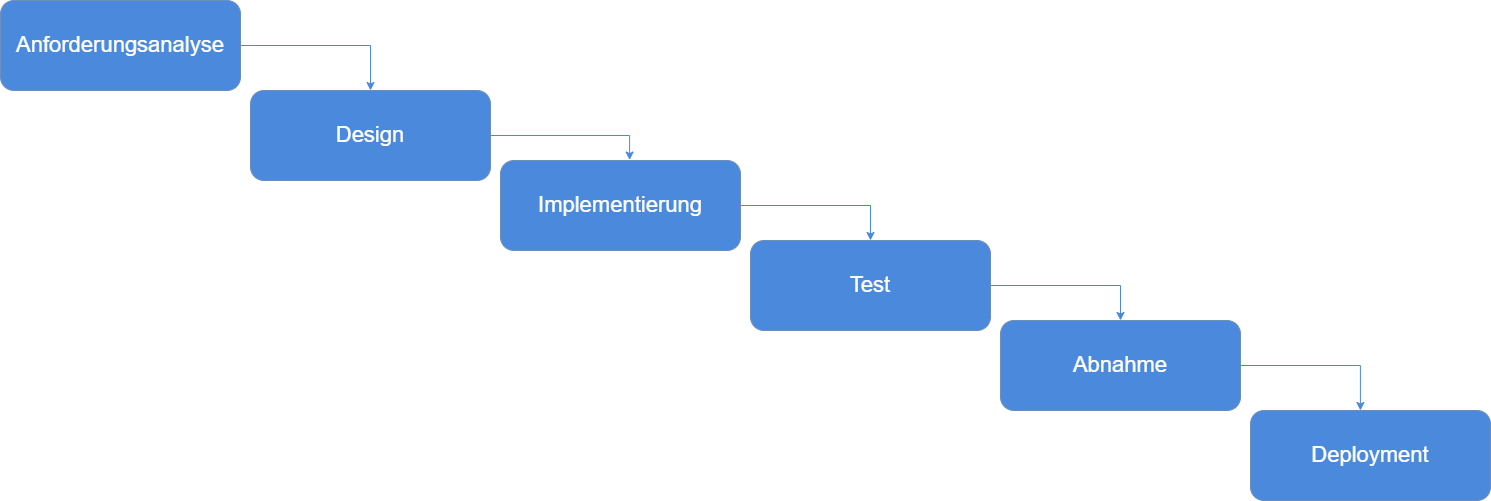
\includegraphics[width=1.1\textwidth]{waterfall.drawio}
\subsection{ Datenübersicht}
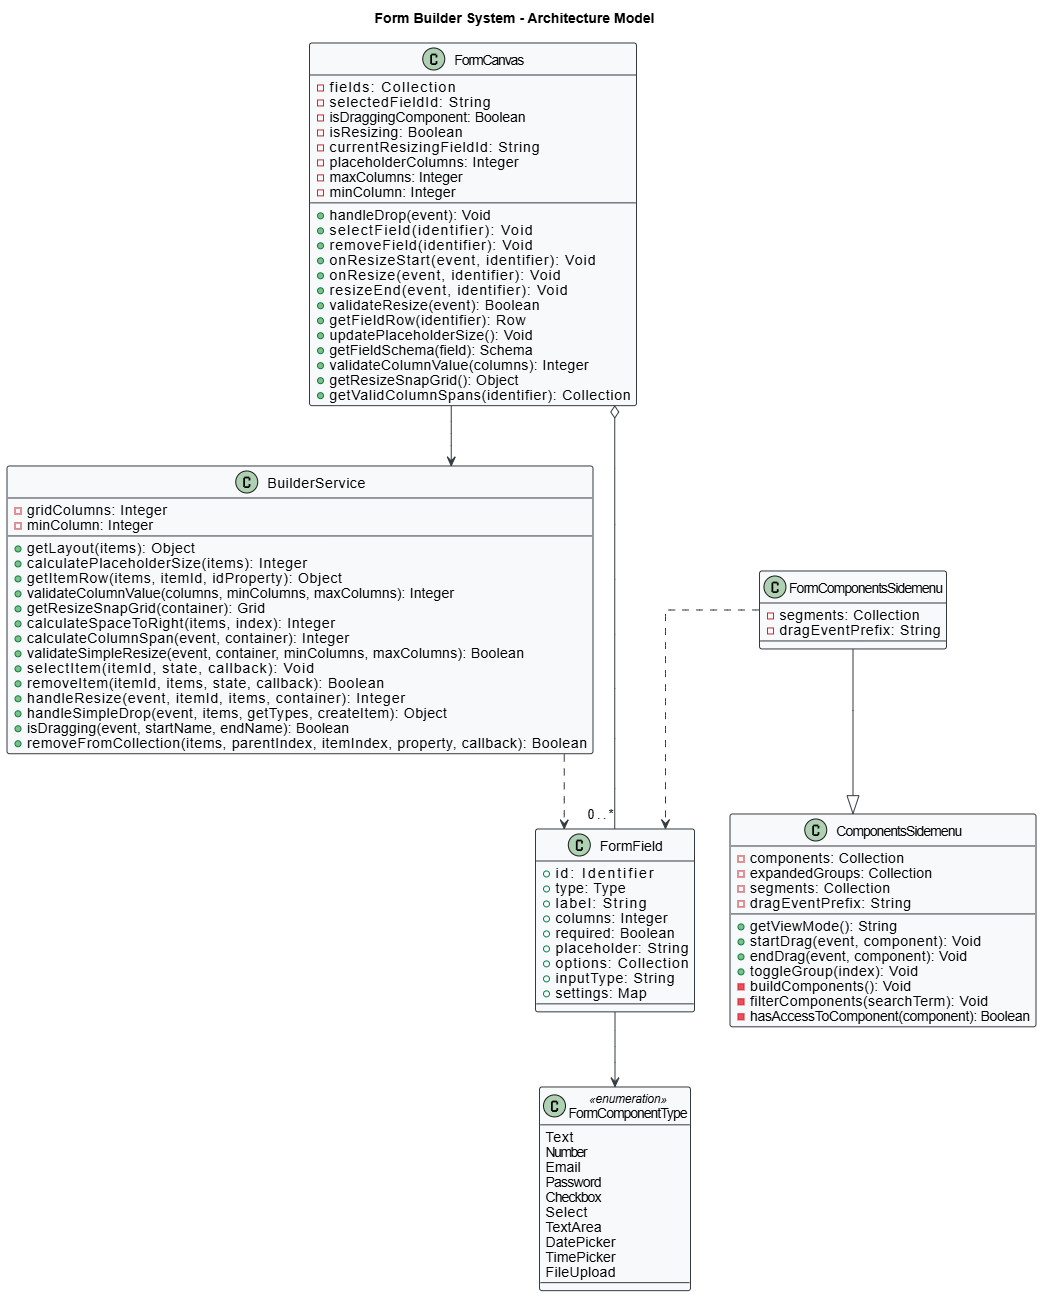
\includegraphics[width=1.1\textwidth]{UML Class digram.drawio}


\newpage
\subsection{ Drag Operation}
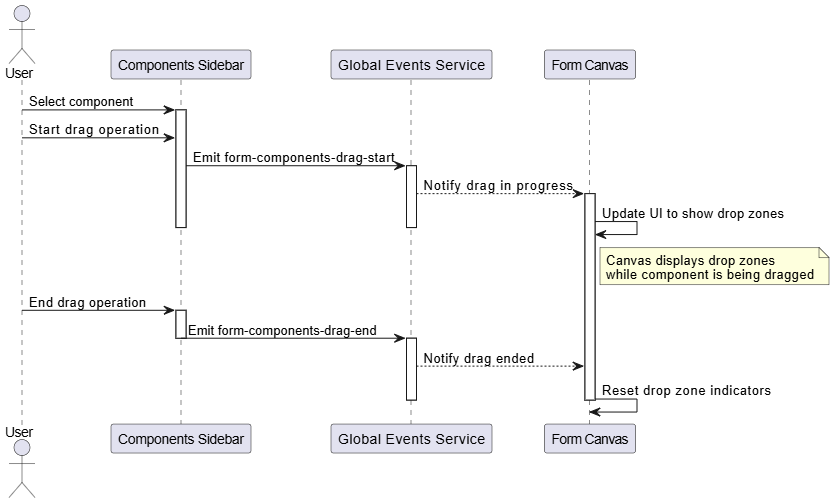
\includegraphics[width=1.1\textwidth]{drag.drawio}
\newpage



\subsection{ Drop Operation}
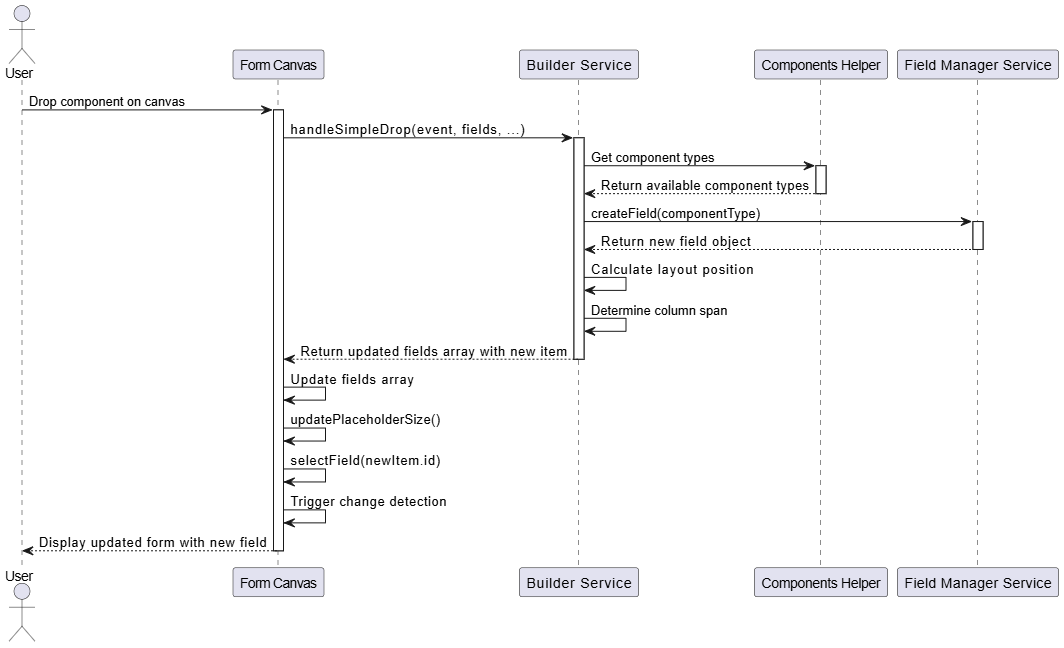
\includegraphics[width=1.1\textwidth]{drop.drawio}
\newpage

\subsection{ Drop and Drop Operation}
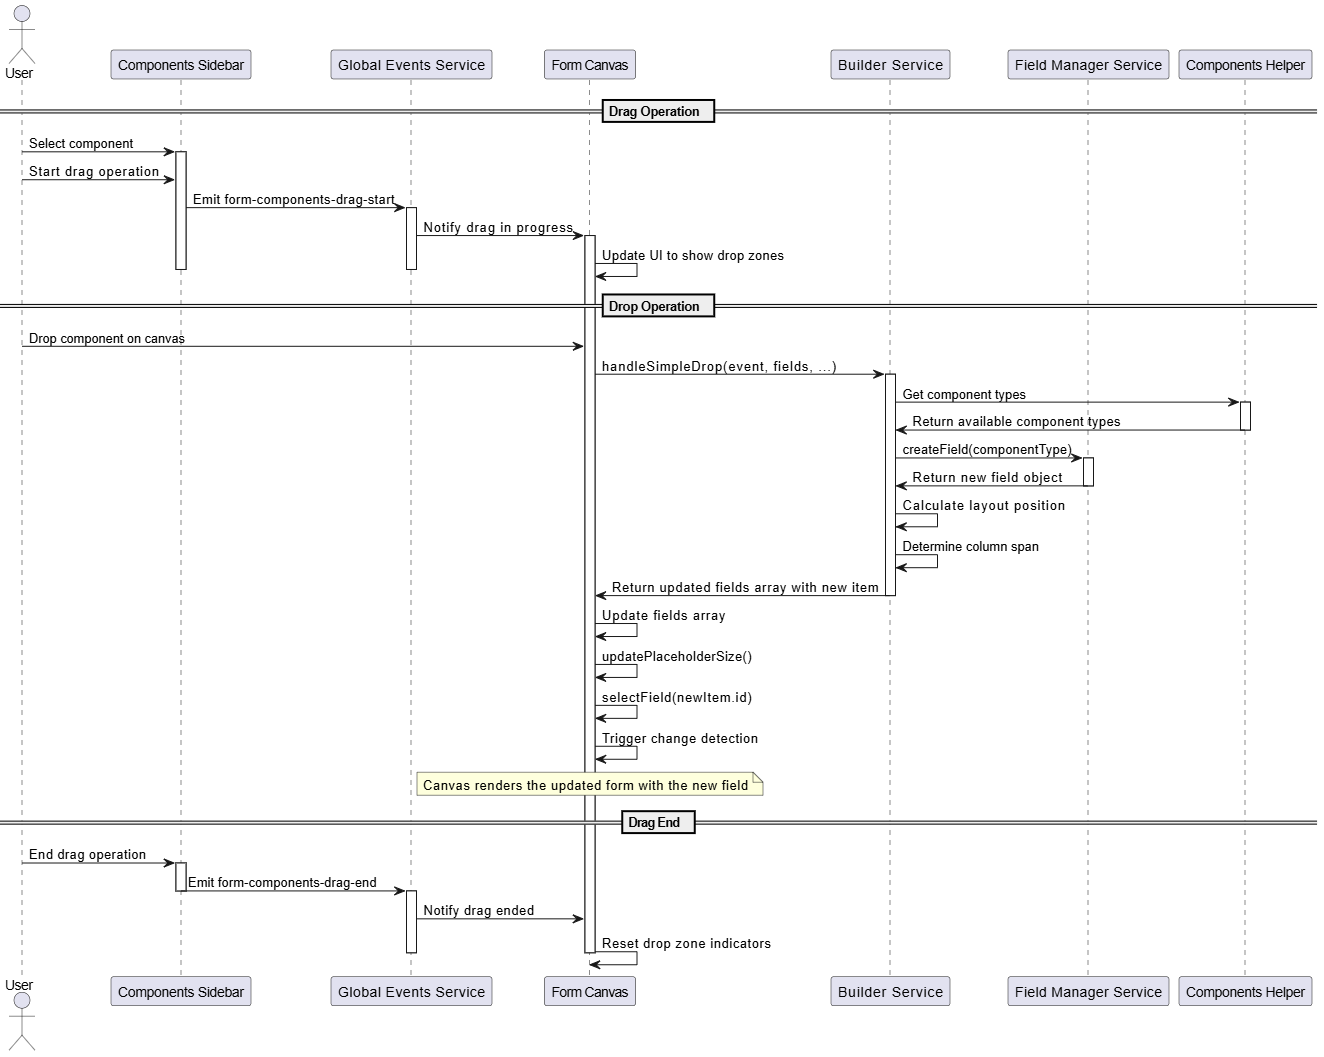
\includegraphics[width=1.1\textwidth]{DragAndDrop.drawio}
\newpage

\section{Code Snippets}
\renewcommand{\lstlistingname}{\texttt{Drop Function in Builder Service}}
\begin{lstlisting}[language=TypeScript, caption={\texttt{handleSimpleDrop} function}]
  /**
   * handler for drop events creating new items
   */
  handleSimpleDrop<T extends { columns: number; id?: string; [key: string]: any }>(
    event: DndDropEvent,
    items: T[],
    getComponentTypes: () => string[],
    createItemFn: (type: string) => T,
    maxColumns: number = 12,
  ): { updatedItems: T[]; newItem: T | null } {
    const updatedItems = [...items];
    if (!event?.data?.type?.startsWith('component:')) {
      return { updatedItems, newItem: null };
    }
    const componentType = event.data.type.split(':')[1];
    if (!getComponentTypes().includes(componentType)) {
      return { updatedItems, newItem: null };
    }
    const newItem = createItemFn(componentType);
    if (updatedItems.length === 0) {
      newItem.columns = Math.min(6, maxColumns);
      updatedItems.push(newItem);
      return { updatedItems, newItem };
    }
    const layout = this.getLayout(updatedItems);
    const lastRow = layout.rows[layout.rows.length - 1];
    const remainingColumns = maxColumns - lastRow.usedColumns;
    if (remainingColumns >= 3) {
      const lastItemIndex = lastRow.itemIndexes[lastRow.itemIndexes.length - 1];
      newItem.columns = Math.min(remainingColumns, 6);
      updatedItems.splice(lastItemIndex + 1, 0, newItem);
    } else {
      newItem.columns = Math.min(6, maxColumns);
      updatedItems.push(newItem);
    }
    return { updatedItems, newItem };
  }
\end{lstlisting}
\renewcommand{\lstlistingname}{\texttt{Aufruf von handleSimpleDrop in Canvas Kompopnente }}
\begin{lstlisting}[language=TypeScript, caption={\texttt{handleSimpleDrop} function}]
  onDrop(event: DndDropEvent): void {
    const result = this.builderService.handleSimpleDrop(
      event,
      this.fields,
      () => this.componentsHelper.getComponentTypes(),
      (type) => this.fieldManager.createField(type as FormComponentType),
      this.MAX_COLUMNS,
    );
    if (!result.newItem) return;
    this.fields = result.updatedItems;
    this.updatePlaceholderSize();
    this.selectField(result.newItem.id);
    this.cdr.detectChanges();
  }
}
\end{lstlisting}




\newpage
\renewcommand{\lstlistingname}{\texttt{Resize Function in Builder Service}}
\begin{lstlisting}[language=TypeScript, caption={\texttt{handleSimpleDrop} function}]
 /**
   * resize end handler
   */
  handleResize<T extends { columns: number; [key: string]: any }>(
    event: ResizeEvent,
    itemId: string,
    items: T[],
    designerViewportElement: ElementRef<HTMLDivElement>,
    idProperty: string = 'id',
    maxColumns: number = this.MIN_COLUMN,
    minColumns: number = this.GRID_COLUMNS,
  ): number {
    if (!designerViewportElement?.nativeElement || !event.rectangle?.width) {
      return -1;
    }

    // Find the item
    const itemIndex = items.findIndex((item) => item[idProperty] === itemId);
    if (itemIndex === -1) {
      return -1;
    }
    // Calculate new column span based on the resize event
    const containerWidth = designerViewportElement.nativeElement.clientWidth;
    const columnWidth = containerWidth / maxColumns;
    const newColumnSpan = Math.round(Number(event.rectangle.width) / columnWidth);
    // Constrain to valid range
    const columnSpan = Math.max(minColumns, Math.min(newColumnSpan, maxColumns));
    // Update the item's columns
    items[itemIndex].columns = columnSpan;
    return columnSpan;
  }
\end{lstlisting}

\renewcommand{\lstlistingname}{\texttt{Aufruf von handleResize in Canvas Kompopnente}}
\begin{lstlisting}[language=TypeScript, caption={\texttt{handleSimpleDrop} function}]
  resizeEnd(event: ResizeEvent, fieldId: string): void {
    if (!this.designerViewportElement?.nativeElement || !event.rectangle?.width) {
      this.isResizing = false;
      this.currentlyResizingFieldId = undefined;
      return;
    }
    const newColumnSpan = this.builderService.handleResize(
      event,
      fieldId,
      this.fields,
      this.designerViewportElement,
      'id',
      this.MAX_COLUMNS,
      this.MIN_COLUMN,
    );
    if (newColumnSpan > 0) {
      this.updatePlaceholderSize();
    }
    this.isResizing = false;
    this.currentlyResizingFieldId = undefined;
    this.cdr.detectChanges();
  }
\end{lstlisting}









































































































\phantomsection
\addcontentsline{toc}{section}{Literaturverzeichnis}

\begin{thebibliography}{99}
  \bibitem{responsive} Responsive Webdesign. \\
  \url{https://de.wikipedia.org/wiki/Responsive_Webdesign}
  
  \bibitem{angular} Angular.\\
  \url{https://de.wikipedia.org/wiki/Angular}
  
  \bibitem{dotnet} .NET (Plattform). (2023). In Wikipedia. \\
  \url{https://de.wikipedia.org/wiki/.NET_(Plattform)}
  
  \bibitem{jquery} jQuery \\
  \url{https://de.wikipedia.org/wiki/JQuery}
  
  \bibitem{tailwind} Tailwind CSS \\
  \url{https://en.wikipedia.org/wiki/Tailwind_CSS}
  
  \bibitem{rest} Representational State Transfer \\
  \url{https://de.wikipedia.org/wiki/Representational_State_Transfer}
  
  \bibitem{json} JSON\\
  \url{https://de.wikipedia.org/wiki/JSON}
  
  \bibitem{angularservices} Angular Services \\
  \url{https://v17.angular.io/guide/architecture-services}
  
  \bibitem{github} GitHub \\
  \url{https://en.wikipedia.org/wiki/GitHub}
  
  \bibitem{cicd} CI/CD \\
  \url{https://de.wikipedia.org/wiki/CI/CD}
  
  \bibitem{markdown} Markdown \\
  \url{https://de.wikipedia.org/wiki/Markdown}
\end{thebibliography}
\end{document}